% \iffalse meta-comment ------------------------------------------------------
% Copyright 2016 Ross Churchley. Contributions to this package are welcome at
%
%     https://github.com/rchurchley/beamercolortheme-owl
%
%  This work may be distributed and/or modified under the conditions of the
%  LaTeX Project Public License, either version 1.3 of this license or (at
%  your option) any later version. The latest version of this license is in:
%
%     http://www.latex-project.org/lppl.txt
%
%  and version 1.3 or later is part of all distributions of LaTeX version
%  2005/12/01 or later.
% ------------------------------------------------------------------------- \fi
% \iffalse
%<driver> \ProvidesFile{beamercolorthemeowl.dtx}
%<*package>
\NeedsTeXFormat{LaTeX2e}[2005/12/01]
\ProvidesPackage{beamercolorthemeowl}
    [2016/03/15 v0.1.1 A visible colour theme for Beamer presentations]
%</package>
%
%<*driver>
\documentclass[12pt]{ltxdoc}
\usepackage{beamercolorthemeowl}
\IfFileExists{FiraSans.sty}{\usepackage[sfdefault, light]{FiraSans}}{}
\IfFileExists{FiraMono.sty}{\usepackage{FiraMono}}{}
\usepackage[parfill]{parskip}
\usepackage{setspace}
  \onehalfspacing
\usepackage[colorlinks=true, linkcolor=OwlRed, urlcolor=OwlBlue]{hyperref}
\usepackage{graphicx}
\usepackage{geometry}
\usepackage{listings}
  \lstset{%
    basicstyle=\ttfamily\small,
    breaklines=true,
    breakatwhitespace=true,
    gobble=2,
    aboveskip=1em,
    belowskip=1em
  }
  \lstMakeShortInline|

\usepackage{readprov}
\ReadPackageInfos{beamercolorthemeowl}
\begin{document}
  \DocInput{beamercolorthemeowl.dtx}
\end{document}
%</driver>
% \fi
% \CheckSum{0}
%
%
% \title{The \texttt{owl} Beamer colour theme}
% \author{Ross Churchley\\ \texttt{ross@rosschurchley.com}}
% \date{\fileversion, dated \filedate}
%
% \maketitle
%
% \begin{quote}\itshape
% ``The effectiveness of a colour scheme is heavily dependent on the conditions
% you present in. Colours that look nice on a computer screen may be
% invisible projected; colours that stand out in a lit room may strain the
% eyes in a dark room. If possible, you should carefully choose from Beamer's
% wide variety of colour themes to find one that fits your presentation's
% individual needs.''
% \end{quote}
%
% The above paragraph would be excellent advice, except for one thing ---
% only a handful of pre-selected colour themes are publicly available for
% Beamer. The vast majority of Beamer presentations use one of the
% \href{https://mpetroff.net/files/beamer-theme-matrix/}{built-in colour
% themes}, which are effective in some conditions but inadequate in others.
% The goal of this package is to reduce the number of situations you
% find yourself without any good colour options. |owl| is a flexible dark or
% light colour theme designed for maximum readability in environments where
% most themes fall flat.
%
%
% \clearpage
% \singlespacing
% \tableofcontents
% \onehalfspacing
%
% \section{Usage}
%
% Once you have downloaded and installed the |beamercolorowl| package, using
% it is a piece of cake:
%
% \begin{lstlisting}
%  \usecolortheme{owl}
% \end{lstlisting}
%
% Unlike many Beamer themes, |owl| defaults to a ``dark'' theme with white
% text on a black background.
% This is particularly recommended for presentations with low ambient lighting,
% where it has the most advantages (see Section~\ref{sec:bg}).
%
% If you expect to present in a brightly-lit room or with a weak projector,
% you may wish to use to use the |snowy| option to use black text on a white
% background:
%
% \begin{lstlisting}
%  \usecolortheme[snowy]{owl}
% \end{lstlisting}
%
% In addition to setting the colour scheme of your slides, |owl| redefines the
% redefines the basic colour names |red|, |green|, |blue|, |yellow|,
% |violet|, |brown|, |orange|, and |cyan| to hues that are more visible when
% when displayed by some projectors. If you do not want these colour names to
% be redefined, use the |cautious| option when loading |owl|:
%
% \begin{lstlisting}
%  \usecolortheme[cautious]{owl}
% \end{lstlisting}
%
% In either case, |owl|-defined colours will be available as |OwlRed|,
% |OwlGreen|, |OwlBlue|, and so forth.
%
%
%
% \iffalse Package options
  \RequirePackage{etoolbox}
  \newtoggle{snowy}
  \newtoggle{cautious}
  \@ifclassloaded{beamer}{
    \DeclareOptionBeamer{snowy}{\toggletrue{snowy}}
    \DeclareOptionBeamer{cautious}{\toggletrue{cautious}}
    \ProcessOptionsBeamer
  }{}
% \fi
%
%
%
% \section{The Background}
% \label{sec:bg}
%
% \subsection{Dark background (default)}
%
% By default, |owl| is a dark colour theme. This isn't just because owls are
% usually nocturnal --- a black background actually offers several advantages.
%
% \begin{itemize}
%   \item In low-light environments, a dark background helps to reduce
%         eye strain and focus attention on the content of your slides.
%   \item Laser pointers are more visible against dark backgrounds. It's also
%         easier to interact directly with your slides when the projector
%         isn't shining as bright a light at your eyes and body.
%   \item With a perfectly black background, there is no visual distinction
%         between the frame margin and the surrounding projector screen.
%         Because of this, less space needs to be dedicated to the margins of
%         each slide; you could afford to use a larger font size, say, to
%         increase visibility of the content.
% \end{itemize}
%
% There are a few caveats to using a black background. First and foremost,
% when applying a black background to an existing presentation, it is
% important to check that your figures and charts look all right.
% Diagrams created with TikZ or PGFPlots are easily adjusted to a new colour
% scheme; images generated from external tools may need to be re-exported,
% edited with an image editing program, or
% \href{http://tex.stackexchange.com/questions/34110/}{preprocessed} with the
% |convert| utility.
%
%
% \subsection{Light background}
%
% If your presentation or environment prevent you from using a dark
% background, but you still want to use the other colours in |owl|'s palette,
% you can use the |snowy| option to switch to a light theme. (Snowy owls, of
% course, are diurnal and have white plumage.)
%
% \begin{lstlisting}[title={\itshape Implementation}]
  \@ifclassloaded{beamer}{
    \iftoggle{snowy}{
      \setbeamercolor{normal text}{fg=black, bg=white}
    }{
      \setbeamercolor{normal text}{fg=white, bg=black}
    }
  }{}
% \end{lstlisting}
%
%
%
% \section{The Colours}
%
% The projectors I encounter regularly tend to have very bright green channels
% and dim red and blue channels: the default |green| is sometimes so
% bright as to be indistinguishable from white, while even pure |red| and
% |blue| are still too dim to tell apart from black. The |owl| colour theme
% provides a basic colour palette that attempts to compensate for this.
%
% \subsection{Primary colours}
%
% \begin{description}
%   \item[\textcolor{OwlBlue}{OwlBlue}]
%        is a greenish blue, bright enough to be legible on a dark
%        background.
%   \item[\textcolor{OwlGreen}{OwlGreen}]
%        is a darker green than the default, and with a slightly yellower hue
%        to help distinguish it from |OwlBlue|.
%   \item[\textcolor{OwlRed}{OwlRed}]
%        is a pinkish magenta, which combines the (individually dim) red and
%        blue channels on the projector to produce enough light to be legible.
%   \item[\textcolor{OwlYellow}{OwlYellow}]
%        is a gold colour of moderate brightness.
% \end{description}
%
% In addition to being distinguishable from white and black, these colours have
% been chosen to be as distinct as possible from one another. Even so, it is
% always a good idea to take care when selecting colours for your presentation.
% For audience members with red-green colour vision deficiencies, |OwlGreen|
% and |OwlYellow| may be difficult to tell apart, while |OwlRed| may be
% difficult to distinguish from light grey or white.
%
% \begin{lstlisting}[title={\itshape Implementation}]
  \RequirePackage{xcolor}
  \definecolor{OwlRed}{RGB}{    255,  92, 168}
  \definecolor{OwlGreen}{RGB}{   90, 168,   0}
  \definecolor{OwlBlue}{RGB}{     0, 152, 233}
  \definecolor{OwlYellow}{RGB}{ 242, 147,  24}
% \end{lstlisting}
%
% \subsection{Secondary colours}
%
% The |owl| colour theme also provides names for certain combinations of the
% above colours:
% \textcolor{OwlViolet}{\bfseries OwlViolet},
% \textcolor{OwlBrown}{\bfseries OwlBrown},
% \textcolor{OwlOrange}{\bfseries OwlOrange}, and
% \textcolor{OwlCyan}{\bfseries OwlCyan}.
% These should be used sparingly; if possible, it is preferable to use only
% two or three colours in a presentation.
%
% \begin{lstlisting}[title={\itshape Implementation}]
  \colorlet{OwlViolet}{OwlRed!50!OwlBlue}
  \colorlet{OwlBrown}{OwlRed!50!OwlGreen}
  \colorlet{OwlOrange}{OwlRed!50!OwlYellow}
  \colorlet{OwlCyan}{OwlGreen!50!OwlBlue}
% \end{lstlisting}
%
%
% \subsection{Redefines \LaTeX\ colours}
%
% Unless the |cautious| option is used, |owl| redefines the built-in colours
% |red|, |green|, |blue|, |yellow|, |violet|, |brown|, |orange|, and |cyan|
% to the above values. This allows you to create diagrams in TikZ or PGFPlots
% that use |owl|'s legible colours in your presentation but are still easy
% reuse in other contexts.
%
% \begin{lstlisting}[title={\itshape Implementation}]
\iftoggle{cautious}{}{
  \colorlet{red}{OwlRed}
  \colorlet{green}{OwlGreen}
  \colorlet{blue}{OwlBlue}
  \colorlet{yellow}{OwlYellow}
  \colorlet{violet}{OwlViolet}
  \colorlet{brown}{OwlBrown}
  \colorlet{orange}{OwlOrange}
  \colorlet{cyan}{OwlCyan}
}
% \end{lstlisting}
%
%
%
% \section{Implementation: Beamer colour definitions}
%
% The Beamer colours set by |owl| all derive from the definitions of
% |normal text|, |alerted text|, and |example text|. This makes it easy for
% you to tweak the theme; for example, you can add
% \begin{lstlisting}
% \setbeamercolor*{alerted text}{fg=OwlBlue}
% \setbeamercolor*{example text}{fg=OwlYellow}
% \end{lstlisting}
% to your preamble to change the highlight colours of the theme.
%
% \begin{lstlisting}
  \@ifclassloaded{beamer}{
    \setbeamercolor*{alerted text}{
      fg=OwlRed
    }
    \setbeamercolor*{example text}{
      fg=OwlGreen
    }
% \end{lstlisting}
%
% \subsection{Title page}
% \begin{lstlisting}
    \setbeamercolor*{title}{
      use=normal text,
      fg=normal text.fg
    }
    \setbeamercolor*{title in sidebar}{
      use=normal text,
      fg=normal text.fg
    }
    \setbeamercolor*{titlelike}{
      use=normal text,
      parent=normal text.fg
    }
    \setbeamercolor*{author}{
      use=normal text,
      parent=normal text.fg
    }
    \setbeamercolor*{date}{
      use=normal text,
      parent=normal text.fg
    }
    \setbeamercolor*{institute}{
      use=normal text,
      parent=normal text.fg
    }
% \end{lstlisting}
%
% \subsection{Palettes}
% \begin{lstlisting}
    \setbeamercolor*{structure}{
      use=normal text,
      fg=normal text.fg!50!normal text.bg
    }
    \setbeamercolor*{palette primary}{
      use=normal text,
      fg=normal text.fg!90!normal text.bg,
      bg=normal text.bg!90!normal text.fg
    }
    \setbeamercolor*{palette secondary}{
      use=normal text,
      fg=alerted text.fg!75!normal text.bg,
      bg=normal text.bg!90!normal text.fg
    }
    \setbeamercolor*{palette tertiary}{
      use=normal text,
      fg=example text.fg!75!normal text.bg,
      bg=normal text.bg!90!normal text.fg
    }
    \setbeamercolor*{palette quaternary}{
      use=normal text,
      fg=normal text.fg!75!normal text.bg,
      bg=normal text.bg!90!normal text.fg
    }
    \setbeamercolor*{sidebar}{
      use=normal text,
      fg=normal text.fg!80!normal text.bg,
      bg=normal text.bg!80!normal text.fg
    }
    \setbeamercolor*{palette sidebar primary}{
      use=palette primary,
      parent=palette primary
    }
    \setbeamercolor*{palette sidebar secondary}{
      use=palette primary,
      parent=palette primary
    }
    \setbeamercolor*{palette sidebar tertiary}{
      use=palette quaternary,
      parent=palette quaternary
    }
    \setbeamercolor*{palette sidebar quaternary}{
      use=palette quaternary,
      parent=palette quaternary
    }
    \setbeamercolor*{frametitle}{
      use=palette primary,
      parent=palette primary
    }
% \end{lstlisting}
%
% \subsection{Blocks}
% \begin{lstlisting}
    \setbeamercolor*{block title}{
      use=normal text,
      fg=normal text.fg,
      bg=
    }
    \setbeamercolor{block body}{
      bg=
    }
    \setbeamercolor*{block title alerted}{%
        use={block title, alerted text},
        fg=alerted text.fg,
        bg=block title.bg
    }
    \setbeamercolor*{block title example}{%
        use={block title, example text},
        fg=example text.fg,
        bg=block title.bg
    }
    \setbeamercolor*{block body alerted}{
      use=block body,
      parent=block body
    }
    \setbeamercolor*{block body example}{
      use=block body,
      parent=block body
    }
% \end{lstlisting}
%
%
% \subsection{Tweaks to Beamer}
%
% Since |owl| does not set a background colour for |block| environments,
% it also prevents the built-in themes from adding drop shadows to blocks.
% Finally, |owl| fixes a pet peeve of mine and disables the navigation symbols
% that often appear at the bottom right of Beamer presentations.
%
% \begin{lstlisting}
    \def\beamer@themerounded@shadow{false}
    \setbeamertemplate{navigation symbols}{}
  }{}
% \end{lstlisting}
%
%
%
% \section{License and contributions}
%
% |owl| may be distributed and/or modified under the conditions of the
% \href{http://www.latex-project.org/lppl.txt}{LaTeX Project Public License}
% version 1.3 or later. The Current Maintainer of this work is Ross Churchley
% (|ross@rosschurchley.com|), who welcomes contributions to the package
% \href{https://github.com/rchurchley/beamercolortheme-owl}{on GitHub}.
%
% The goal of |owl| is to provide colours that are as visible as possible,
% even in unfavourable presenting conditions. This can be challenging to test
% with only one pair of eyes and a handful of projectors!
% If you have used |owl| or seen it used, we would greatly appreciate your
% opinion on how it performed. Please open a GitHub Issue or privately email
% the Current Maintainer with as much of the following information as you can:
%
% \begin{itemize}
%   \item The version of |owl| used.
%   \item The Beamer theme, if any, that was used together with |owl|.
%   \item Whether |owl| was used as a dark or light theme.
%   \item Details on the room (auditorium, large room, small room, \ldots)
%   \item Details on the lighting conditions (brightly lit, dark, windows,
%         \ldots)
%   \item Details, if known, on the reporter's vision (glasses, colour
%         deficiencies, \ldots)
%   \item Your opinion on:
%         \begin{itemize}
%           \item whether normal text was visible against the background.
%           \item whether the provided colours (|OwlRed|, |OwlBlue|, etc) were
%                 legible against the background.
%           \item whether the provided colours (|OwlRed|, |OwlBlue|, etc) were
%                 distinguishable from each other and from the normal text
%                 colour.
%         \end{itemize}
% \end{itemize}
%
% We also welcome technical feedback and bug reports in the form of
% GitHub Issues and pull requests.
%
%
% \clearpage
% \newgeometry{margin=1in}
% \section{Examples}
%
%   \begin{center}
%   \textit{Pittsburgh}
%
%   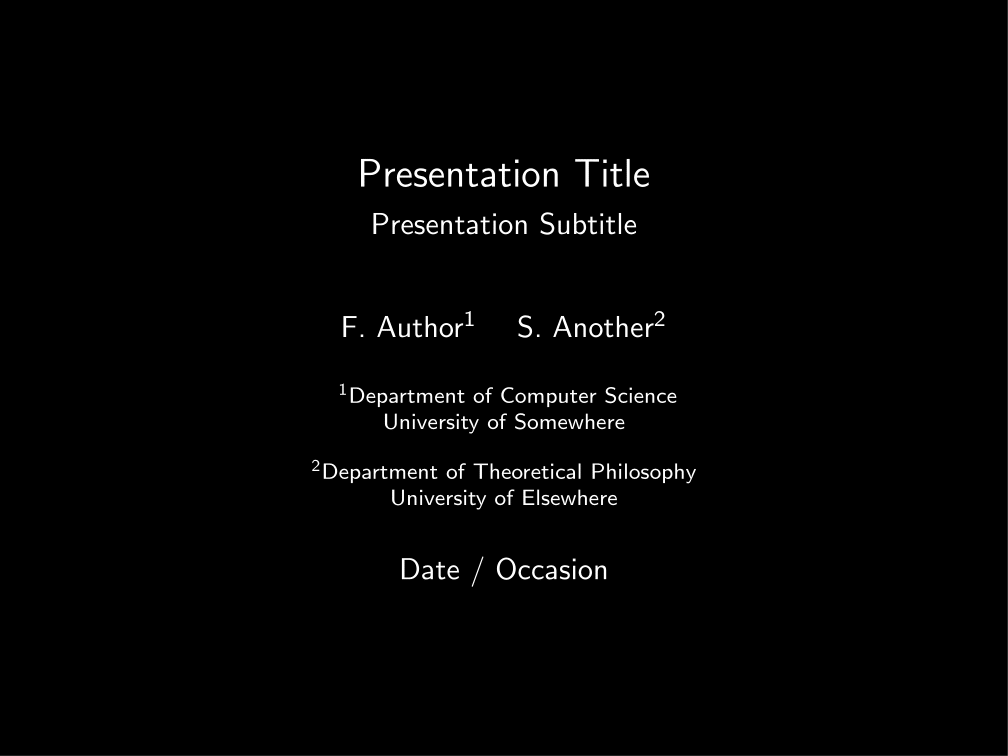
\includegraphics[scale=0.2]{ex/Pittsburgh-dark/Pittsburgh-owl-1.png}
%   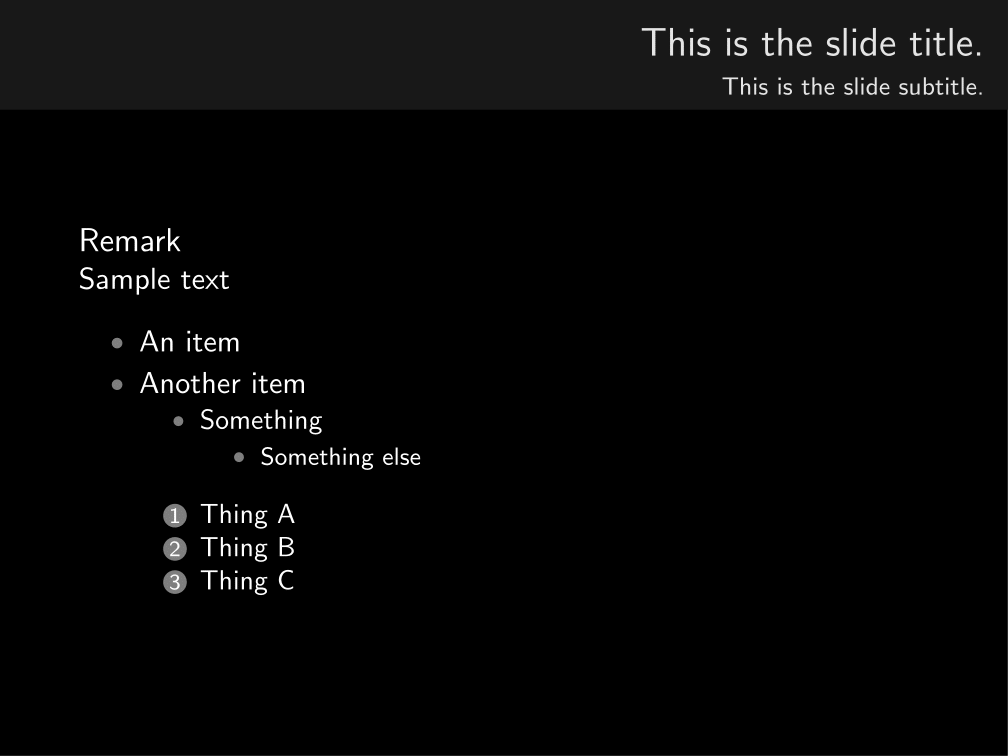
\includegraphics[scale=0.2]{ex/Pittsburgh-dark/Pittsburgh-owl-2.png}
%
%   \textit{Hannover}
%
%   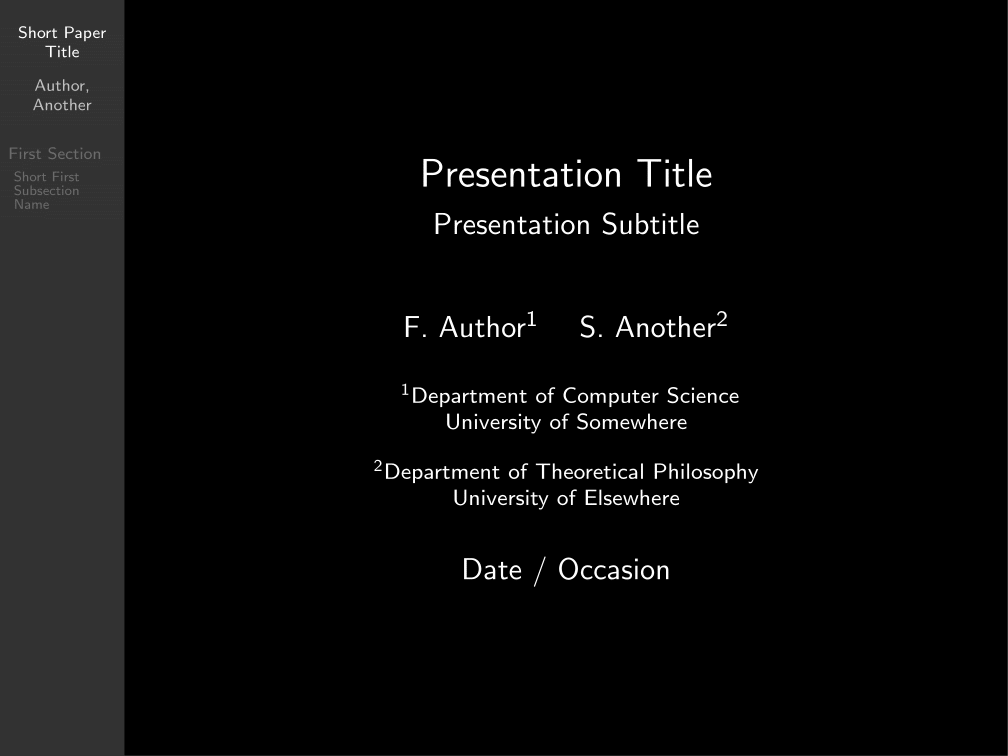
\includegraphics[scale=0.2]{ex/Hannover-dark/Hannover-owl-1.png}
%   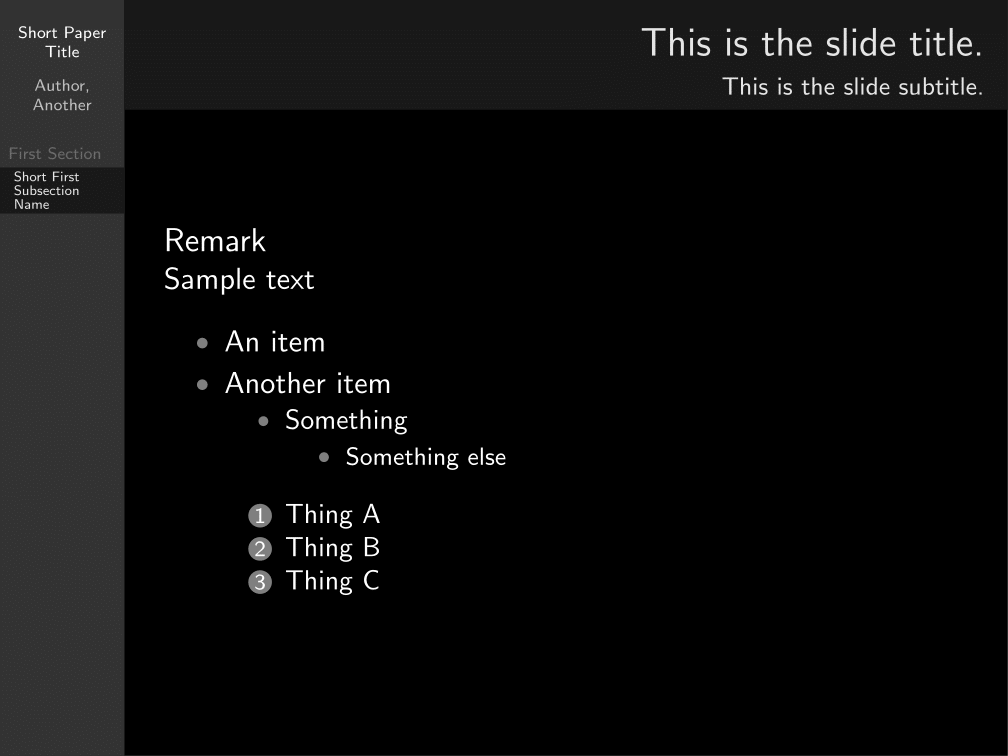
\includegraphics[scale=0.2]{ex/Hannover-dark/Hannover-owl-2.png}
%
%   \href{https://github.com/matze/mtheme}{\itshape metropolis}
%
%   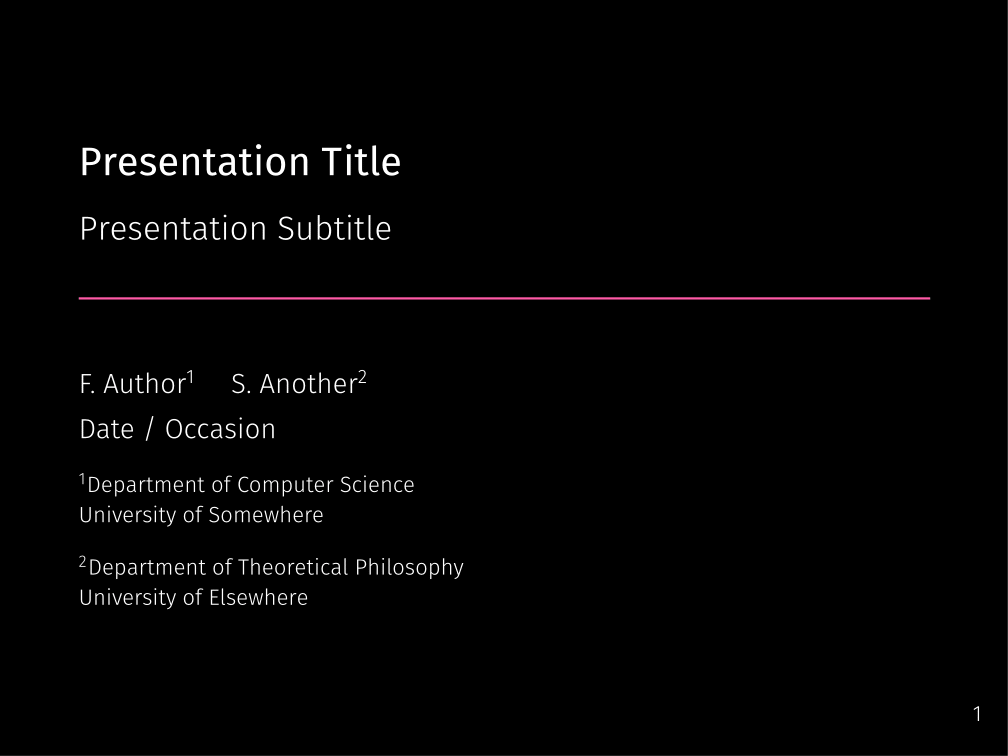
\includegraphics[scale=0.2]{ex/metropolis-dark/metropolis-owl-1.png}
%   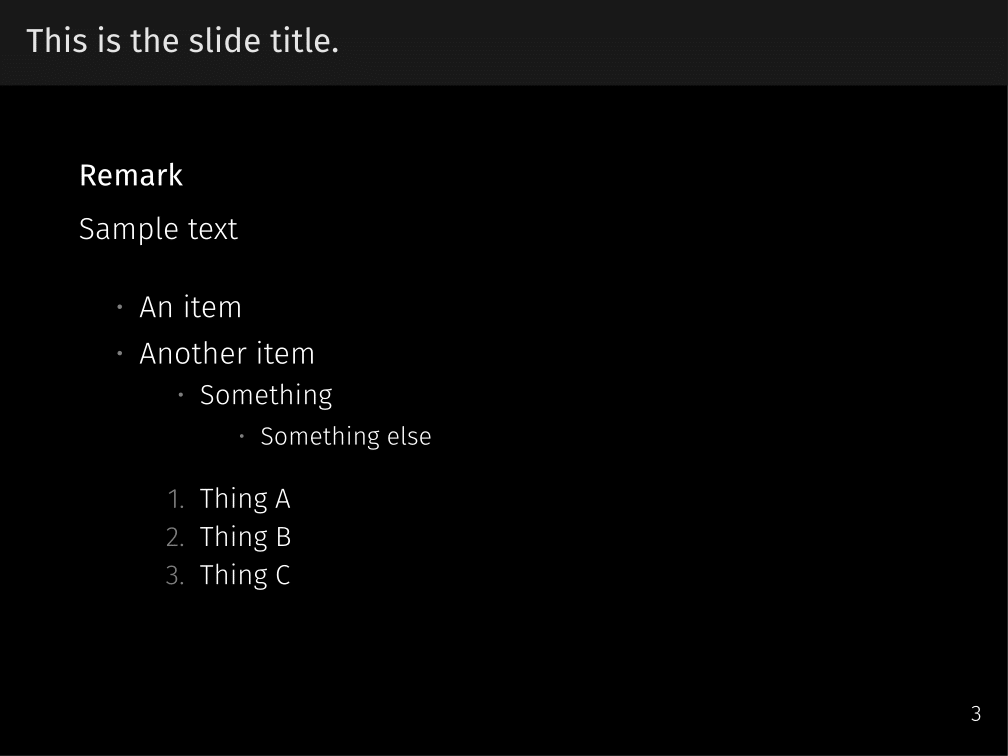
\includegraphics[scale=0.2]{ex/metropolis-dark/metropolis-owl-2.png}
%
%   \clearpage
%
%   \textit{Pittsburgh} (|snowy owl|)
%
%   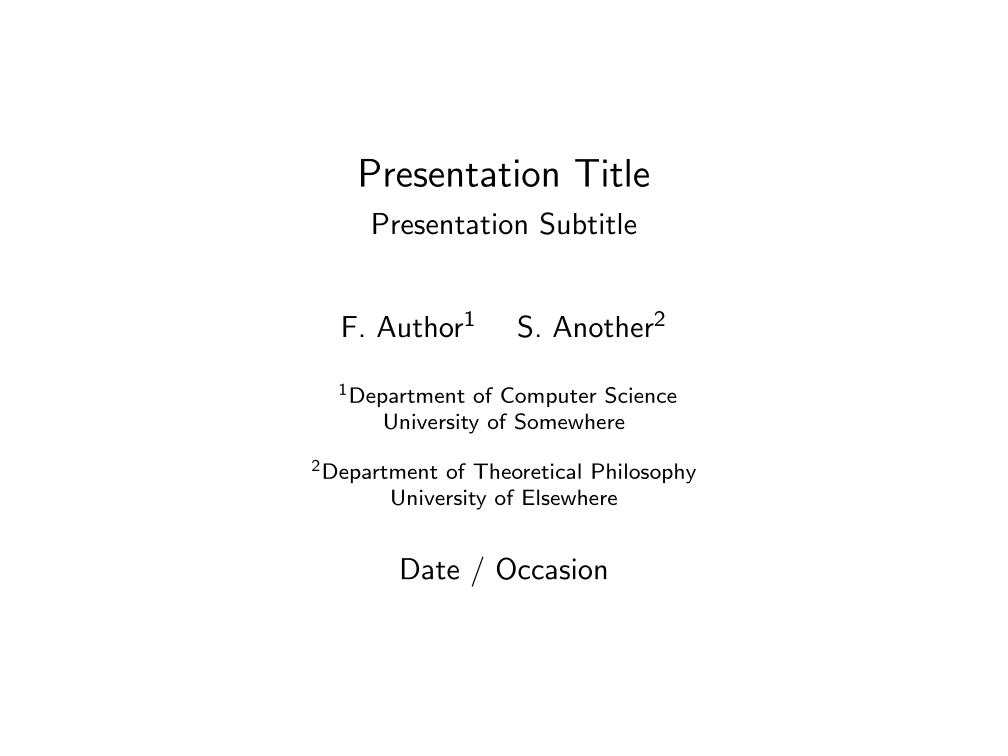
\includegraphics[scale=0.2]{ex/Pittsburgh-light/Pittsburgh-owl-1.png}
%   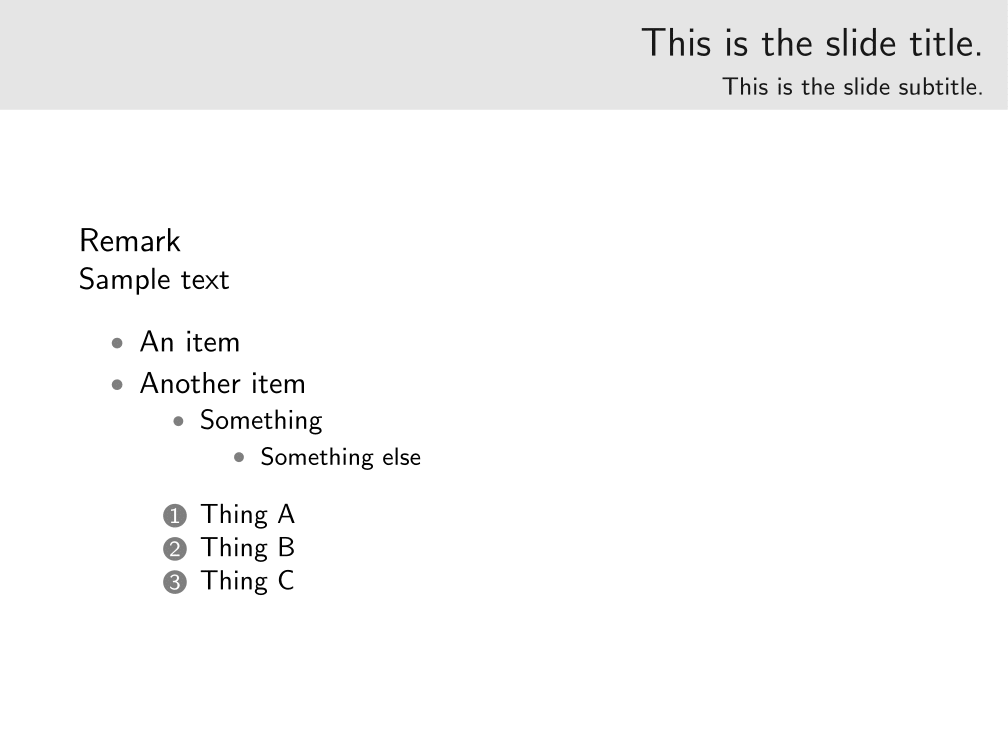
\includegraphics[scale=0.2]{ex/Pittsburgh-light/Pittsburgh-owl-2.png}
%
%   \textit{Hannover} (|snowy owl|)
%
%   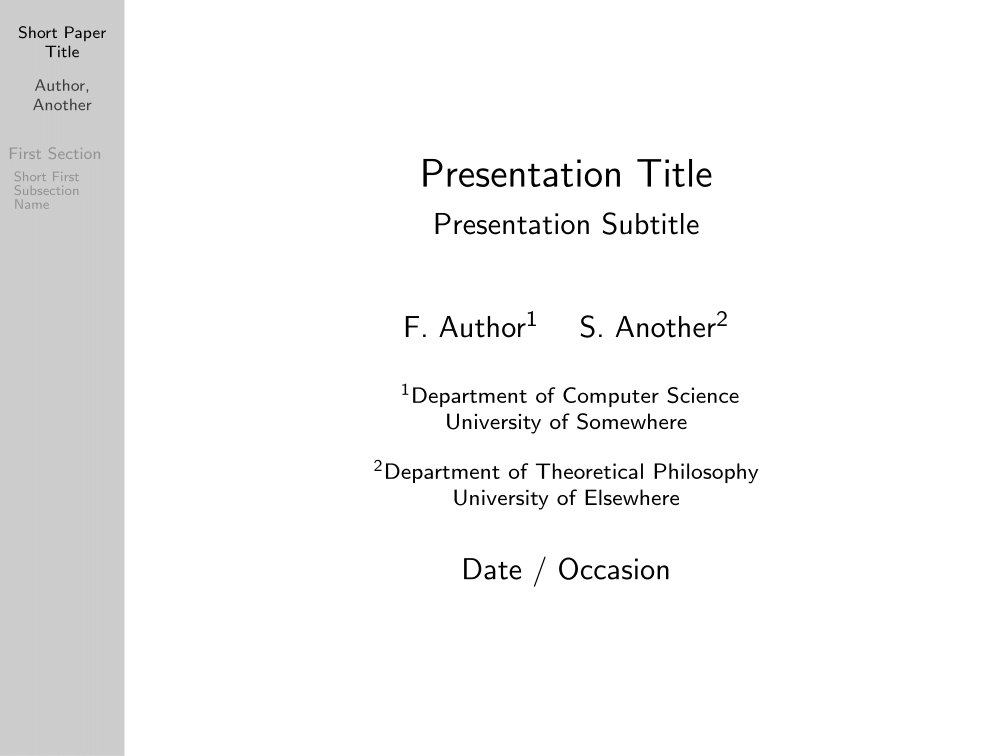
\includegraphics[scale=0.2]{ex/Hannover-light/Hannover-owl-1.png}
%   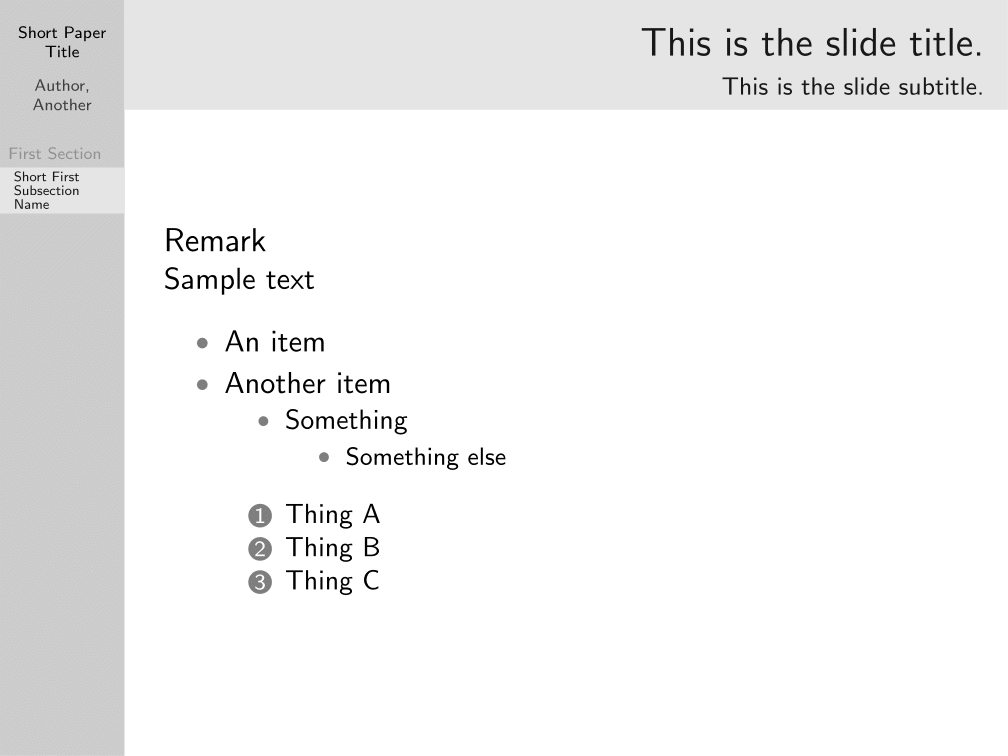
\includegraphics[scale=0.2]{ex/Hannover-light/Hannover-owl-2.png}
%
%   \href{https://github.com/matze/mtheme}{\itshape metropolis} (|snowy owl|)
%
%   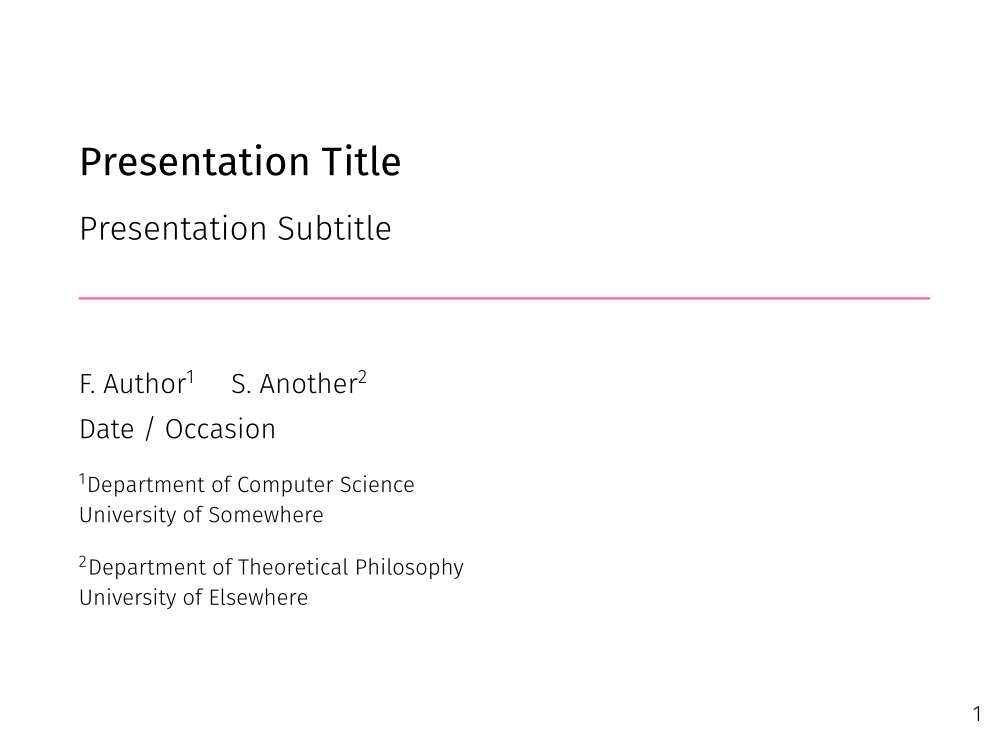
\includegraphics[scale=0.2]{ex/metropolis-light/metropolis-owl-1.png}
%   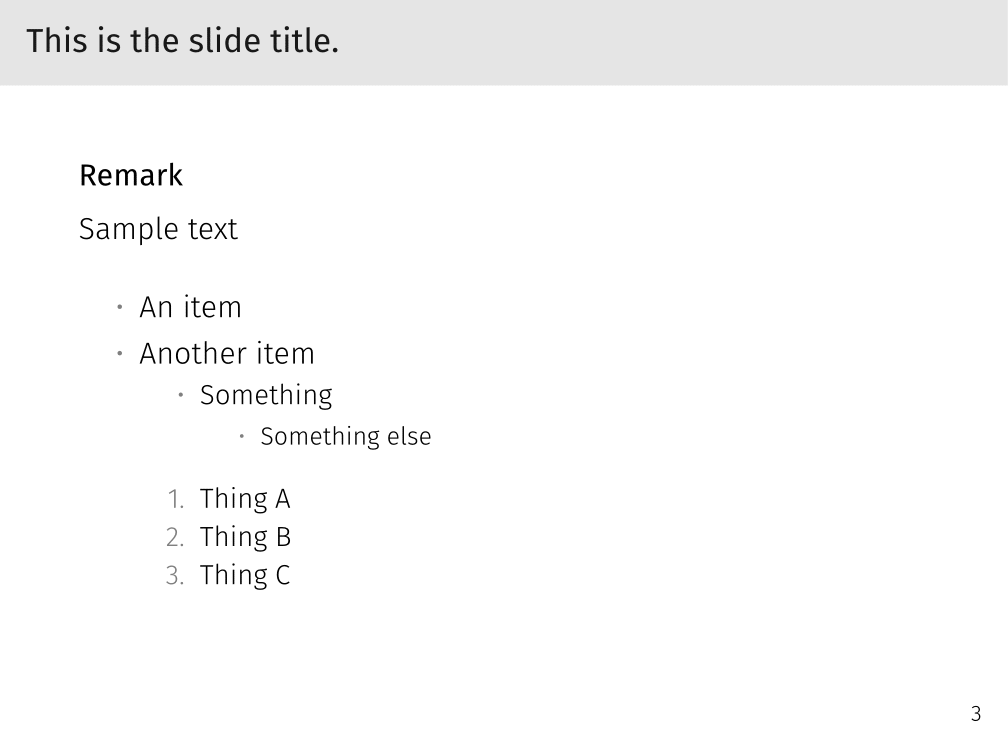
\includegraphics[scale=0.2]{ex/metropolis-light/metropolis-owl-2.png}
%   \end{center}
%
% \restoregeometry
% \clearpage
%
% \Finale
\endinput
